% This is samplepaper.tex, a sample chapter demonstrating the
% LLNCS macro package for Springer Computer Science proceedings;
% Version 2.20 of 2017/10/04
%
\documentclass[runningheads]{llncs}
%
\usepackage{graphicx}
\usepackage{amssymb}
\usepackage{algorithmicx}
\usepackage{algorithm2e}
\usepackage[utf8]{inputenc}
\usepackage{subfig}
% Used for displaying a sample figure. If possible, figure files should
% be included in EPS format.
%
% If you use the hyperref package, please uncomment the following line
% to display URLs in blue roman font according to Springer's eBook style:
% \renewcommand\UrlFont{\color{blue}\rmfamily}

\begin{document}
%
\title{Visual Analytics of Large Bipartite Networks assisted by Multilevel Strategies\thanks{Supported by FAPESP, project 2017/05838-3}}
%
\titlerunning{Multilevel Visualization of Bipartite Networks}
% If the paper title is too long for the running head, you can set
% an abbreviated paper title here
%
\author{Renato Fabbri\orcidID{0000-0002-9699-629X} \and
Alan Valejo \and
Maria Cristina Ferreira de Oliveira\orcidID{0000-0002-4729-5104}}
%
\authorrunning{R. Fabbri et al.}
% First names are abbreviated in the running head.
% If there are more than two authors, 'et al.' is used.
%
\institute{University of São Paulo, São Carlos SP, BR\\
\email{renato.fabbri@gmail.com},
\email{alanvalejo@gmail.com},
\email{cristina@icmc.usp.br}\\
\url{http://conteudo.icmc.usp.br/pessoas/cristina/}}
%
\maketitle
%
\begin{abstract}
% The abstract should briefly summarize the contents of the paper in
% 150--250 words.
  It is a well established fact that bipartite, or two-layer, networks are pervasive
  in model real-world phenomena and that they play fundamental roles in
  graph theory.
  Multilevel strategies have been developed for optimization tasks,
  and for the visualization of simple (``unipartite'') networks,
  but their employment for visualizing bipartite networks were not found by the authors.
  In this work, we present advances in the use of multilevel strategies for the
  visualization of bipartite networks,
  allowing for interactive and intuitive navigation of such structures and visual mappings of large datasets.
  More specifically, we developed a visual analytics web interface in which
  a parametrizable simplification of
  bipartite networks are obtained through the application of coarsening algorithms.
  The resulting networks are then presented to the user,
  providing a genuine route for the ``overview first - focus on demand''
  process on the analysis of the underlying data, in which the analyst
  selects supervertices or whole network sectors for more detailed observation,
  i.e. performs requests for the interface to display 
  specific structures in less simplified settings.
  Moreover, the application is useful for the further development multilevel strategies themselves
  e.g. by the specification of vertices to guide the coarsening processes and
  the examination of the resulting multilevel hierarchy.

\keywords{Network visualization \and Multilevel strategies \and Visual analytics \and Big data \and Complex networks \and Data visualization.}
\end{abstract}
%
\section{Introduction}
The visualization of large-scale networks poses challenges both in terms of computational costs
and of effective presentation of the information to the user~\cite{tang,staudt}.
These issues may be aggravated in the case of bipartite networks,
due to their sparsity and topological complexities~\cite{alan1}.
Bipartite networks are comprised of two partitions of nodes,
called ``layers'',
and links are not incident between nodes in the same partition.
Such network type arises very often and naturally from the representation
of relations among two kinds objects,
e.g. documents and terms or authors~\cite{doc,sci,movie}, or patient and gene~\cite{gene}.
Furthermore, real-world networks are often bipartite, and most unipartite networks
are projections of bipartite networks or exhibit bipartite properties~\cite{guillaume0,guillaume}.
In order to assist the visualization and navigation of large networks, one possibility is the use of
multilevel strategies, which consist on the employment of incremental coarsening of the original
network to obtain a sequence of simplified representations.
Multilevel strategies are most traditionally used for executing complex algorithms
on large-scale networks by the application of the algorithm on a smaller
version of the network~\cite{alan2,ml2}.
The employment of multilevel strategies for the visualization of simple (i.e. ``unipartite'')
networks have been reported, but their exploitation for visualizing bipartite networks
was not found by the authors, as described in the next subsection.
Accordingly, we present a system for the visualization of bipartite networks using
multilevel strategies developed for bipartite networks.
The system consists on presenting a simplified version of the network to the user, which then
requests for supervertices (or collections of them) to be uncoarsened and visualized in more detail.

This paper is organized as follows: in Section~\ref{rel} the related work is examined,
while in~\ref{nom} are selected remarks about the vocabulary.
The method is delineated in Section~\ref{des} and
the software implementation is then described in Section~\ref{sof}.
Results and discussion are in~\ref{res}.
Finally, Section~\ref{con} holds concluions and further work envisioned.

\subsection{Related work}\label{rel}
%%%
% artigos que devemos citar pelo histórico científico
% da estratégia ML, da visualização ML
% e os que devemos citar pelo ML em redes bipartidas
% e desenvolvidos no ICMC
Multilevel strategies have been employed to visualize unipartite networks~\cite{u1,u2,u3,u4,u5,u6,u7}.
Also, the aggregation of clusters have been reported, and comprises an approach that resembles
the coarsening procedure in creating simplified representations of the original network~\cite{a1,a2,a3,a4,a5,a6}.
Even so, the authors are not aware of previous reports on the use of multilevel strategies
for the visualization and navigation of bipartite networks.
Furthermore, only~\cite{a1,a2,a3,a4,a6} reports on a system suitable for visual analytics, i.e. the other works do not
address data analysis by interactive visual interfaces, including all multilevel strategies for visualization.

\subsection{Nomenclature remarks}\label{nom}
%%%
% level vs layer
% simple and heterogeneous graphs
% multiplex, ?
% multilevel strategies for optimization
% supernode metanode, 
The main vocabulary issue that arises in the context of this article is between
level and layer. Layers are the (two) node partitions of a bipartite network, while levels comprise the sequence
of coarsened networks.
Also, simple or homogeneous networks are opposed to heterogeneous networks, in which there
are more then one type of node.
Bipartite networks may be regarded as an elementary case of heterogeneous networks,
but it has one additional restriction: only nodes of different types are connected.
Another usual concept in this context is that of a multilayer network, in which there are layers,
i.e. partitions of nodes, in addition to nodes and links.
Bipartite networks, in this case, are multilayer networks with only two layers and no intra-layer links, i.e. all the links are inter-layers.
Most importantly, there are many synonyms which are found in this context, e.g. supernodes are also called metanodes or supervertices.
A thorough exposition of the vocabulary is beyond the scope of this article, but
some attention for the issue is helpful to assist searches and newcomers.

\section{Method description}\label{des}
%%%
% mlpb and other methods developed
% arguments for the preferred method (mlpb?)
\subsection{Fundamental concepts}\label{bac}
A bipartite network $G=(V,E)$ consists in a set $V$ of vertices which is partitioned in two subsets
with no links between nodes in the same set, i.e. $\exists\; V_1, V_2:\; V_1\cup V_2 = V,\;V_1\cap V_2 = \emptyset$, and $E\subseteq V_1 \times V_2$.
The variable names are borrowed from more traditional
Graph (network) theory, with Vertices (nodes) and Edges (links).
One may regard the network as $G=(V,E,\sigma,\omega)$,
$\sigma\,:\,V\rightarrow \mathbb{R}^*$ and with $\omega\,:\,E \rightarrow \mathbb{R}^*$,
where $\sigma(v)$ is the weight of the node $v$ and
$\omega(u,v)$ is the weight of the link $(u,v)$.

A multilevel strategy consists in obtaining a hierarchy of coarsened networks $G_l$, $l$ integer and $l \in [0,L-1]$ where $G_0$ is the original network
and where $|V_i| \leq |V_{i+1}|$.
The coarsening procedures requires two algorithms, the \emph{matching}, that defines the nodes to be collapsed, and the \emph{contraction}, which builds the reduced representation
from the matched nodes.
There are several coarsening algorithms reported in the scientific literature~\cite{}, a few of them
developed for bipartite networks~\cite{}.
An exposition about these algorithms is found on the bibliography~\cite{} and is beyond the scope of this article.
Most importantly, we are interested in coarsening suited for bipartite networks,
as it has yielded simplified networks which present essential topological features
of the original networks,
and such result is perceived in the visualization as hinted in\~cite{alan2} and further shown in
Sections~\ref{des},~\ref{sof} and~\ref{res}.

Visual analytics is the scientific field dedicated to analytical reasoning assisted by interactive visual interfaces~\cite{}.
Therefore, the area is specially concerned with coupling interactive visual representations with sense and decision making.
Of special relevance for the present work, the techniques are most often employed to amplify human capabilities in specific ways,
which includes reducing the search space, enhancing the recognition of patterns and the inference of relationships,
and providing a manipulable medium for the exploration of the information of interest~\cite{}.

\subsection{Multilevel coarsening of bipartite networks}\label{bac}
Before~\cite{alan2}, multilevel approaches were not directly aplicable to bipartite networks.
Such work introduced novel and efficient matching and coarsening algorithms,
and scrutinized their validity for solving optimization problems, dimensionality reduction,
and in the preservation of essential topological features of the original network.
We here describe the outline of such procedures in the context of our visual analytics contribution.

The multilevel optimization is a metaheuristics used to guide,
modify and potentially fix a solution obtained from a target algorithm.
It is divided into three phases: coarsening, solution finding and uncoarsening,
where the solution found in the coarsest network $G_L$ is projected back to the original,
uncoarsened, network $G_0$.
Figure~\ref{mlf} illustrates such process.

\begin{figure}[!h]\centering
 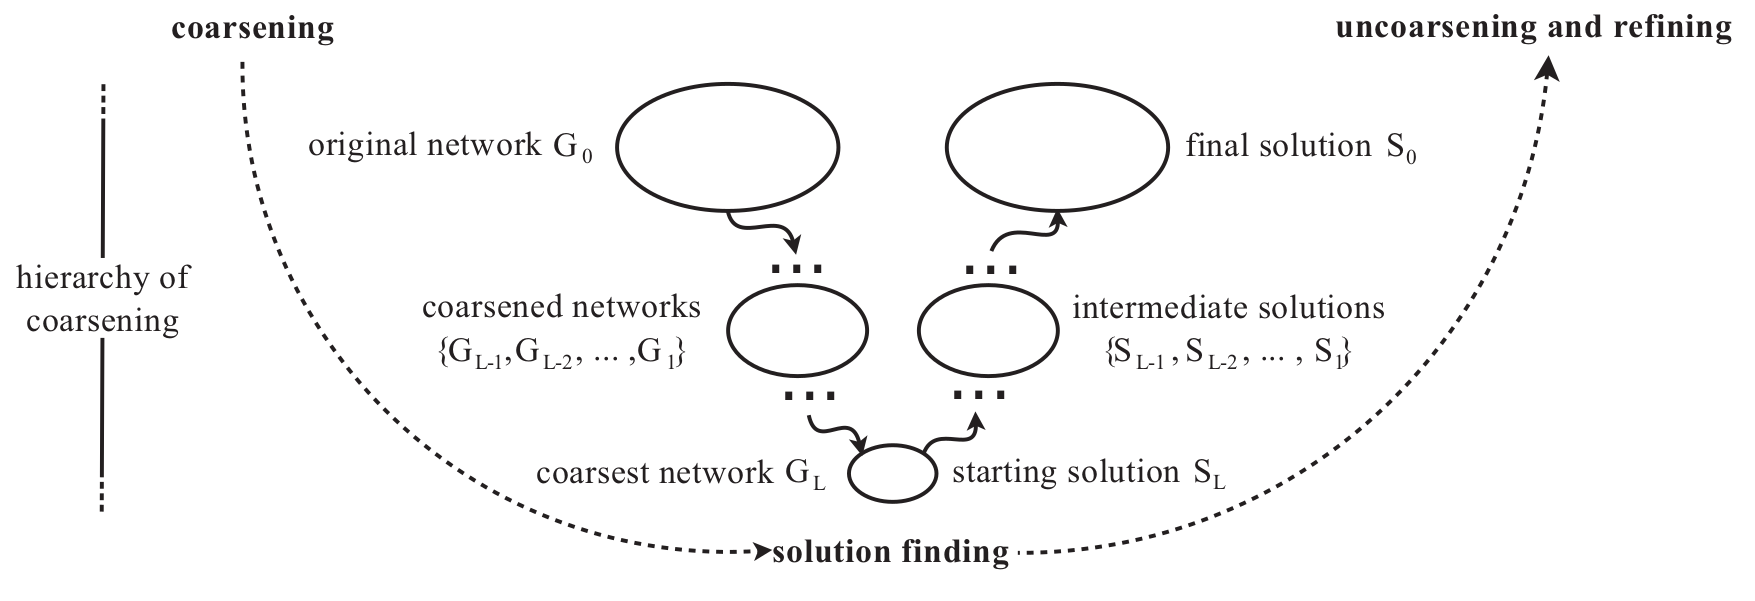
\includegraphics[width=\textwidth]{mlf}
  \caption{Phases of the multilevel optimization.
  A sequence of incrementally reduced networks is obtained in the coarsening phase.
  An initial solution found at the coarsest network, in the solution finding phase,
  is projected back to the initial, uncoarsened, network, in the uncoarsening phase.
  Further details are given in Section~\ref{bac} and specificities related to these
  phases when applied to visual analytics are in Sections~\ref{net} and~\ref{nav}.
  }\label{mlf}
\end{figure}

The coarsening phase results in a sequence of networks $G_l$ from the initial network $G_0$,
on multiple levels of details.
The process is carried out by two algorithms: \emph{matching}, which decides which nodes to merge,
and \emph{contracting}, which achieves the reduced representation from the network and the matching.
In general, pairs of nodes are selected to be merged into supernodes, and
most often a matching $M$ consists in a set of non-adjacent links,
i.e. $\forall\; l_1, l_2 \in M, u \in l_1 \Rightarrow u \notin l_2$.
The heavy-edge mathing, for example, is a matching that fits this canonical description
in attempting to maximize total matching weight, but the matching may not satisfy such restrictions.
Selecting clicks and other larger node sets to be merged into supernodes are possibilites
under development.
%%%
% citar alguem aqui?
For bipartite network, we use the algorithms provided by~\cite{alan2} in which two restrictions
are imposed to the matching:
\begin{itemize}
  \item A node may only match nodes on the same layer.
  \item A node may only match nodes that are reachable by two successive links
    (i.e. the closest possible nodes on the same layer).
\end{itemize}

The matching is followed by the contraction of the network into a coarser form.
Typically, the nodes matched are merged into a supernode
with the weight equal to the sum of the weight of nodes it contains,
and the links incident to such nodes are joined into superlinks among the supervertices,
also with total weight equal to the sum of the weight of the links merged.
The solution finding is usually reasoned about in terms of the computational cost, being much
alleviated in the reduced network.
The uncoarsening is usually performed through the complete hierarchy,
from the coarsest to the original network, with successive refinement of the solutions to
avoid local minima and improve solution quality.
These two phases are substantially different when the multilevel strategy is applied to visualization,
which motivated their separate exposition in the next subsection.

\subsection{Network visualization assisted by multilevel strategies}\label{net}
In applying the multilevel framework to visualization,
the target algorithm is the visual mapping of the network,
i.e. the solution finding phase is the visualization of the network by means of
the reduced representation.
The uncoarsening is performed only on demand, through user requests
to visualize network regions with more detail, thus avoiding unecessary complexity and,
most importantly, avoiding to overload the visualization with information beyond the
cognitive convenience of the user and the computational power that the machine being used
is able to provide for real-time interactivity.

The interactivity is crucial for a number of reasons:
the definition of the uncoarsening phase desired;
for the navigation of the network,
including the access to metadata and changes to the visualization achieved;
for uncoarsening supernodes;
and for tuning the achieved visual mapping status, such as by resizing
and moving nodes.
The overall procedure is delineated in Algorithm~\ref{alg} and further
detailed in Sections~\ref{nav} and~\ref{sof}.


\SetKwData{Matching}{Matching$_b$}
\SetKwData{Contracting}{Contracting$_b$}
\SetKwData{map}{map\_to\_screen}
\SetKwData{trans}{transform\_visual\_mapping}
\SetKwInOut{Return}{Return}
\begin{algorithm}
  \KwIn{\\
  \quad bipartite network: $G$\\
  \quad maximum number of levels: $L \in [0,n] \subset \mathbb{Z}$\\
  \quad reduction factor: $rf \in (0,0.5] \subset \mathbb{R}$.\\
  \quad layers to be coarsened: $layers \in {1,2}$\\
  \quad user command given through the visual interface: $C$
  }
  \KwOut{\\
  \quad Visual mapping of the network: $V$}
  \BlankLine
  $i \leftarrow 1$\;
  \While{$i \le$ layers}{
    $l\leftarrow 1$\;
    \While{$l\leq L$}{
      $M \leftarrow$ \Matching{$G_l$, $i$, $rf$}\;
      $G_{l+1} \leftarrow$ \Contracting{$G_l$, $M$}\;
      increment $l$\;
    }
      increment $i$\;
  }
  $V \leftarrow$ \map{$G_L$}\;
  \While{1}{
    $C\leftarrow$ user command\;
    $V\leftarrow$ \trans{$V$, $C$}\;
  }
  \caption{An algorithmic description of the multilevel strategy adapted for the visualization of bipartite networks.
  The routines {\bf Matching$_b$} and {\bf Contracting$_b$} are any of the matching or contracting
  algorithms suited for bipartite networks, such as described in~\cite{alan2} which are only ones
  currently available to the knowledge of the authors.
  The {\bf map\_to\_screen} routine is performed through the use of a network layout algorithm and
  then the rendering of the network to the screen.
  The visual mapping may then be transformed by the user by requesting uncoarsening of specific supernodes,
  or by other commands not specific to the multilevel strategy, such as requesting metadata exposition, changes to the position of nodes, the color or transparency of nodes and links, zoom and pan,
  or any other operation defined in Section~\ref{sof}.}\label{alg}
\end{algorithm}

\subsection{The navigation pathway}\label{nav}
The abundance of information within large networks makes pertinent the
application of
the ``visual information-seeking mantra'', also known as Shneiderman's mantra:
\emph{overview first, zoom and filter, then details-on-demand}.
This mantra comprises a number of visual design guidelines,
such as the details-on-demand technique, and provides
a very acknowledged framework for designing information visualization applications.
Accordingly, our idealized exploration pathway starts with an overview,
achieved by the mapping the coarsest representation of the network through
standard network layout algorithms for node-link diagrams.
The user may then zoom into specific regions of the network, and then request
details by a number of operations, most importantly:
\begin{itemize}
  \item reposition nodes, exposing linking patterns.
  \item request metadata, such as number of children, the parent in a subsequent level, or the number of neighbors.
  \item request visual mapping of network features, such as node size related to number of neighbors or the number of child nodes it represents.
  \item request the uncoarsening of specific supernodes or any arbitrary group of supernodes.
\end{itemize}

Other operations are convenient to make the visual mapping adequate for the diverse settings possible:
network size, open supervertices, levels exposed, and topological features such as community structures.
The navigations pathway, already as achieved within the software we made available, is illustrated in Figure~\ref{fnav}.

\begin{figure}[!h]\centering
 
\includegraphics[width=0.6\textwidth]{fnav}
  \caption{The navigation pathway of the bipartite network obtained through a multilevel strategy
  and auxiliary tools.
  }\label{fnav}
\end{figure}

\noindent 
\section{Software implementation: mlvis}\label{sof}
%%%
% description of the functionalities/tools implemented,
% of the technologies and libraries used
% optimization of the computational capacity for large networks by
% means of Web GL, triangles for nodes and details on demand
We implemented the framework described in Section~\ref{des} using scientific,
database and web resources,
and made the final result available to the user within a web page
for use through simple mouse-driven actions
and requiring the instalation of no software but a web browser such as Firefox or Google Chrome.
The final result is exemplified in Figures~\ref{fpage0} and~\ref{fpage} and next subsections
describe its functionalities and the technologies used.

\begin{figure}[!h]\centering
 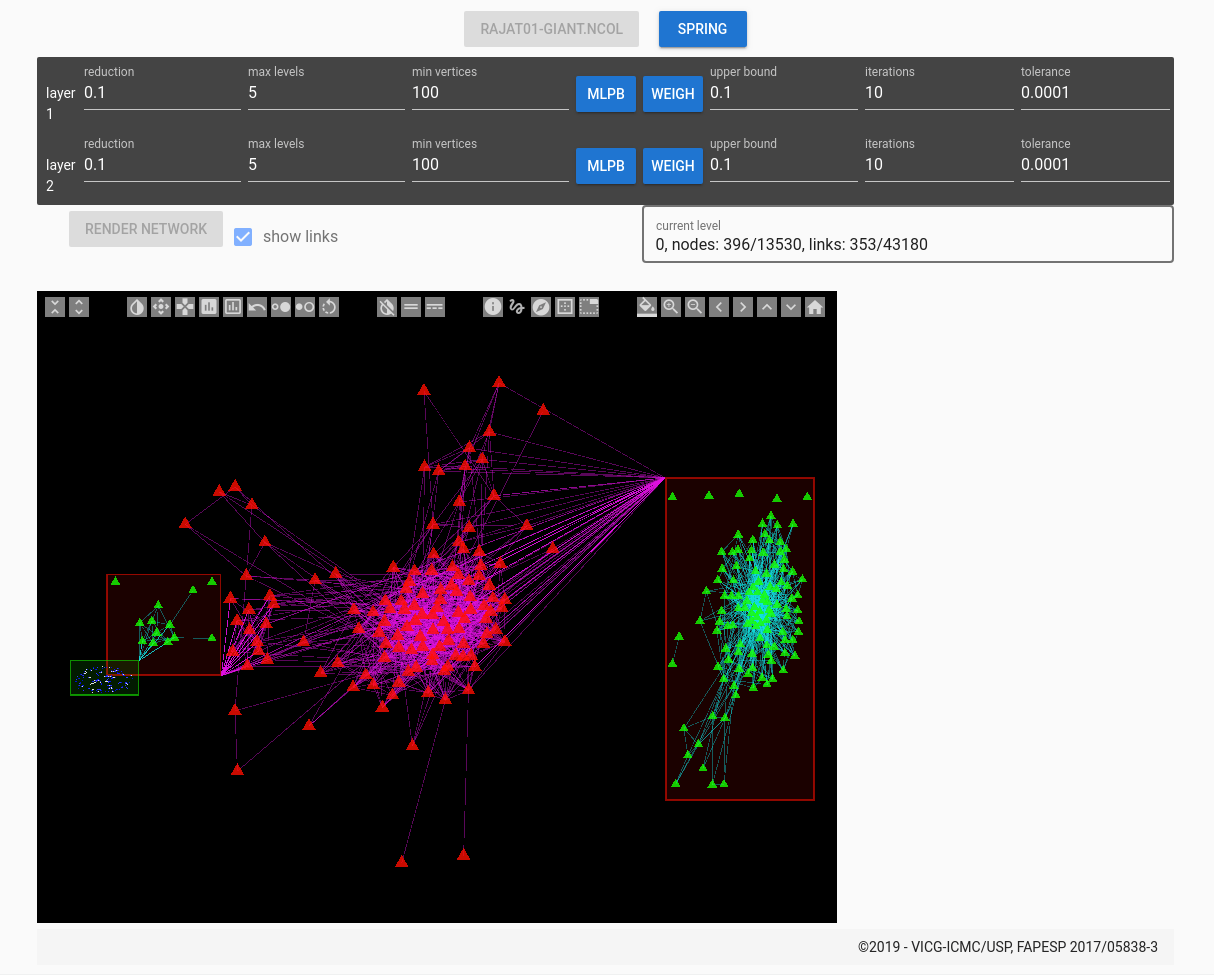
\includegraphics[width=\textwidth]{fpage0}
  \caption{The navigation pathway of the bipartite network obtained through a multilevel strategy
  and auxiliary tools.
  }\label{fpage0}
\end{figure}

\begin{figure}[!h]\centering
 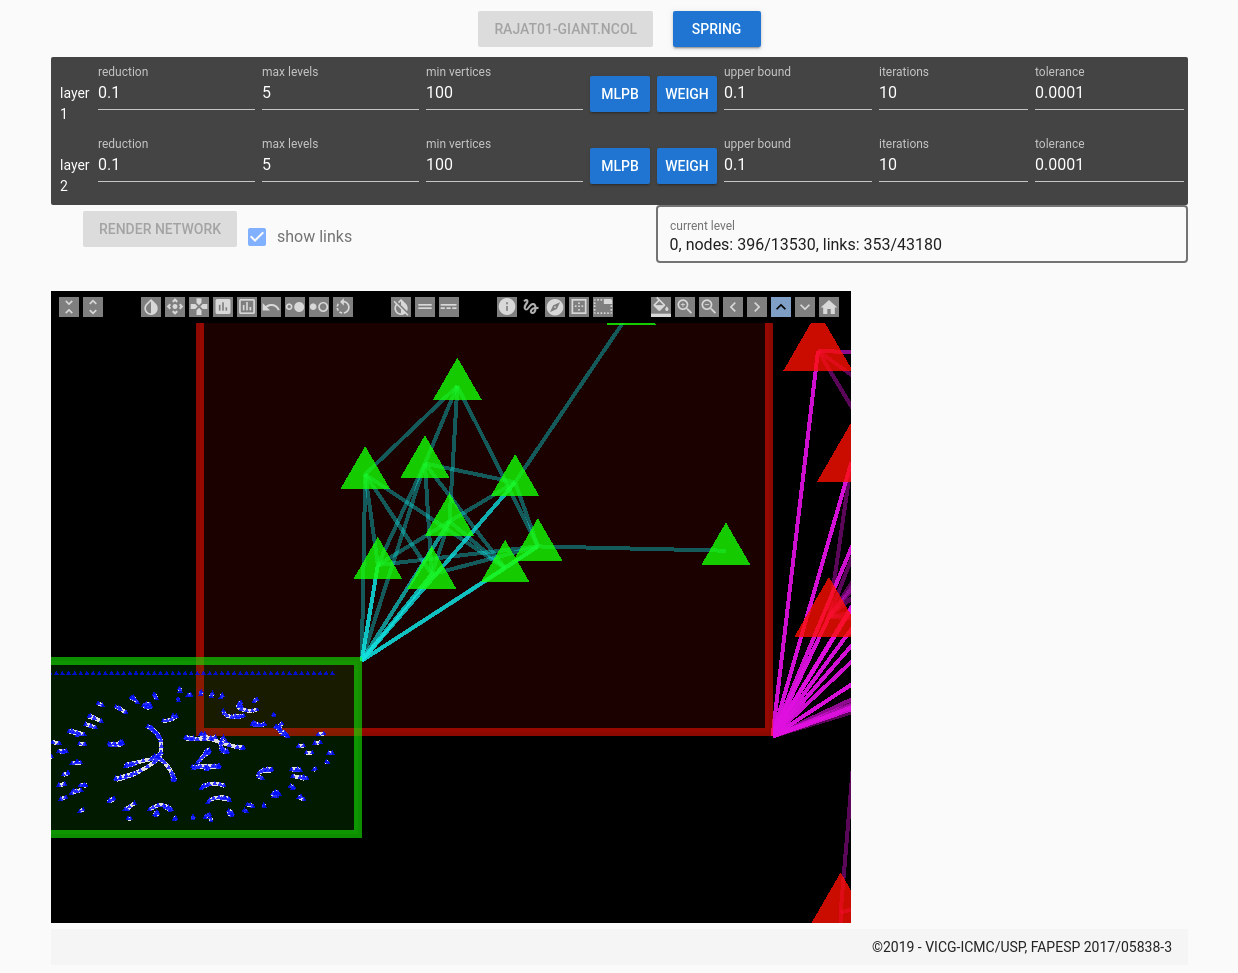
\includegraphics[width=\textwidth]{fpage}
  \caption{The navigation pathway of the bipartite network obtained through a multilevel strategy
  and auxiliary tools.
  }\label{fpage}
\end{figure}

\subsection{The use of mlvis}
% network upload, format.
% layouts available
% algorithms available for coarsening, and their parametrization
% initialization of the visualization: click on render
% tools available and their operation

\subsection{Technologies used within mlvis}
% coarsening algorithms
% flask for server, feather for auxiliary server
% mongodb filesystem for data
% Nuxt/Vue.js for the frontend with heavy use of PIXI.js

\section{Results and discussion}\label{res}
%%%
% consistent use of overview first, details on demand
% a first contribution on ML vis. of bipartite networks
% simple interactivity strategies

% enhancements of the navigation through the use of being-developed coarsening algorithms
% the use of the interface for guiding coarsening (through markers)
% the use of the interface to analyse coarsening results

% technologies used: maybe simpler if using meteor.js
% and simpler to achieve multiuser interactivity

\section{Conclusions and further work}\label{con}
%%%
% extension to multipartite (or heterogeneous) networks.

\bibliographystyle{splncs04}
\bibliography{biblio}
%
% \begin{thebibliography}{8}
% \bibitem{ref_article1}
% Author, F.: Article title. Journal \textbf{2}(5), 99--110 (2016)
% 
% \bibitem{ref_lncs1}
% Author, F., Author, S.: Title of a proceedings paper. In: Editor,
% F., Editor, S. (eds.) CONFERENCE 2016, LNCS, vol. 9999, pp. 1--13.
% Springer, Heidelberg (2016). \doi{10.10007/1234567890}
% 
% \bibitem{ref_book1}
% Author, F., Author, S., Author, T.: Book title. 2nd edn. Publisher,
% Location (1999)
% 
% \bibitem{ref_proc1}
% Author, A.-B.: Contribution title. In: 9th International Proceedings
% on Proceedings, pp. 1--2. Publisher, Location (2010)
% 
% \bibitem{ref_url1}
% LNCS Homepage, \url{http://www.springer.com/lncs}. Last accessed 4
% Oct 2017
% \end{thebibliography}
\end{document}
